\documentclass[titlepage]{report}
\usepackage[backend=biber,style=numeric]{biblatex}
\addbibresource{literature.bib}
\usepackage{caption}
\usepackage{subcaption}
\usepackage{graphicx}
\usepackage[utf8]{inputenc}
\usepackage[T1]{fontenc}
\usepackage{url}
\usepackage{hyphenat}
\usepackage{glossaries}
\usepackage{array}
\usepackage{calc}
\usepackage{booktabs}
\usepackage{hyperref}
\usepackage{listings}
% \usepackage{xcolor} https://tex.stackexchange.com/q/466147
\usepackage{bytefield}
\usepackage{float}
\usepackage{eurosym}
\usepackage{tabu}
\usepackage{caption}
\usepackage{csquotes}
\lstset{%
    frame=tb,
    tabsize=4,
    numbers=left,
    breaklines=true,
}
\setcounter{biburllcpenalty}{9001}
\makeglossaries{}
\newglossaryentry{ima}
{%
    name={IMA},
    description={Computer network airborne system},
    first={Integrated Modular Avionics (IMA)},
    long={Integrated Modular Avionics}
}
\newglossaryentry{dima}
{%
    name={DIMA},
    description={Distributed computer network airborne system},
    first={Distributed Integrated Modular Avionics (DIMA)},
    long={Distributed Integrated Modular Avionics}
}
\newglossaryentry{apex}
{%
    name={APEX},
    description={APplication/EXecutive Interface},
    first={APplication/EXecutive Interface (APEX)},
    long={APplication/Executive Interface}
}
\newglossaryentry{coex}
{%
    name={COEX},
    description={COre/EXecutive Interface},
    first={COre/EXecutive Interface (APEX)},
    long={COre/Executive Interface}
}
\newglossaryentry{arinc}
{%
    name={ARINC},
    description={Aeronautical Radio Incorporated},
    first={Aeronautical Radio Incorporated (ARINC)},
    long={Aeronautical Radio Incorporated}
}
\newglossaryentry{aeec}
{%
    name={AEEC},
    description={Airlines Electronic Engineering Committee},
    first={Airlines Electronic Engineering Committee (AEEC)},
    long={Airlines Electronic Engineering Committee}
}
\newglossaryentry{lru}
{%
    name={LRU},
    description={Line-Replaceable Unit},
    first={Line-Replaceable Unit (LRU)},
    long={Line-Replaceable Unit},
    plural={LRUs},
    firstplural={Line-Replacable Units (LRUs)}
}
\newglossaryentry{lrm}
{%
    name={LRM},
    description={Line-Replaceable Module},
    first={Line-Replaceable Module (LRM)},
    long={Line-Replaceable Module},
    plural={LRMs},
    firstplural={Line-Replacable Modules (LRMs)}
}
\newglossaryentry{arinc429}
{%
    name={ARINC 429},
    description={ARINC standard for a global data bus in aviation},
    first={ARINC 429 standard},
    long={ARINC 429 standard}
}
\newglossaryentry{arinc629}
{%
    name={ARINC 629},
    description={ARINC standard for a global computer bus in aviation},
    first={ARINC 629 standard},
    long={ARINC 629 standard}
}
\newglossaryentry{arinc650}
{%
    name={ARINC 650},
    description={ARINC standard for IMA packaging and interfaces},
    first={ARINC 650 standard},
    long={ARINC 650 standard}
}
\newglossaryentry{arinc651}
{%
    name={ARINC 651},
    description={ARINC report that provides guidelines for a maintenance strategy for IMA-equipped airplanes},
    first={ARINC 651 report},
    long={ARINC 651 report}
}
\newglossaryentry{arinc653}
{%
    name={ARINC 653},
    description={ARINC standard for space and time partitioning},
    first={ARINC 653 standard},
    long={ARINC 653 standard}
}
\newglossaryentry{arinc659}
{%
    name={ARINC 659},
    description={ARINC standard for a backplane data bus},
    first={ARINC 659 standard},
    long={ARINC 659 standard}
}
\newglossaryentry{RTCA}
{%
    name={RTCA},
    description={Radio Technical Commission for Aeronautics (RTCA)},
    first={Radio Technical Commission for Aeronautics (RTCA)},
    long={Radio Technical Commission for Aeronautics}
}
\newglossaryentry{do178b}
{%
    name={DO-178B},
    description={Certification for safety-critical software by the RTCA},
    first={DO-178B},
    long={DO-178B}
}
\newglossaryentry{do178c}
{%
    name={DO-178C},
    description={Certification for safety-critical software by the RTCA (replaces DO-178B)},
    first={DO-178C},
    long={DO-178C}
}
\newglossaryentry{us}
{%
    name={US},
    description={United States of America. Short: United States},
    first={United States (US)},
    long={United States}
}
\newglossaryentry{io}
{%
    name={I/O},
    description={input and output},
    first={input and output (I/O)},
    long={input and output}
}
\newglossaryentry{cpu}
{%
    name={CPU},
    description={The CPU consists of registers for fast computation and an Algorithmic Logic Unit (ALU)},
    first={Central Processing Unit (CPU)},
    long={Central Processing Unit}
}
\newglossaryentry{ram}
{%
    name={RAM},
    description={RAM is very fast memory for temporary storing data},
    first={Random Access Memory (RAM)},
    long={Random Access Memory}
}
\newglossaryentry{nist}
{%
    name={NIST},
    description={United States institute for promoting innovation and industrial competitiveness},
    first={National Institute of Standards and Technology (NIST)},
    long={National Institute of Standards and Technology}
}
\newglossaryentry{saas}
{%
    name={SaaS},
    description={},
    first={Software as a Service (SaaS)},
    long={Software as a Service}
}
\newglossaryentry{paas}
{%
    name={PaaS},
    description={},
    first={Platform as a Service (PaaS)},
    long={Platform as a Service}
}
\newglossaryentry{iaas}
{%
    name={IaaS},
    description={},
    first={Infrastructure as a Service (IaaS)},
    long={Infrastructure as a Service}
}
\newglossaryentry{hsd}
{%
    name={HSD},
    description={},
    first={Horizontal Situation Display (HSD)},
    long={Horizontal Situation Display}
}
\newglossaryentry{arp4754}
{%
    name={ARP4754},
    description={Guideline for the development of aircraft systems by SAE International},
    first={Aerospace Recommended Practic (ARP) 4754},
    long={Aerospace Recommended Practic 4754}
}
\newglossaryentry{dal}
{%
    name={DAL},
    description={Design Assurance Level},
    first={Design Assurance Level (DAL)},
    long={Design Assurance Level}
}
\newglossaryentry{idal}
{%
    name={IDAL},
    description={Item Development Assurance Level},
    first={Item Development Assurance Level (IDAL)},
    long={Item Development Assurance Level}
}



\title{From the Cloud to the Clouds: Taking Integrated Modular Avionics on a New Level with Cloud-Native Technologies}
\author{Christian Rebischke\\
Clausthal University of Technology\\
Student ID: 432108 \\
E-Mail: Christian.Rebischke@tu-clausthal.de}
\begin{document}
\maketitle
\chapter*{Acknowledgement}
\chapter*{Statutory Declaration}
This master thesis is submitted in partial fulfilment of the requirements for the Clausthal
University of Technology. I hereby declare that this dissertation is my own work and
contains nothing which is the outcome of work done in collaboration with others,
except as specified in the text and acknowledgements. The contributions of any other
supervisors to this thesis are made with specific reference.
\\
\\
Clausthal-Zellerfeld, \today
\\
\\
Christian Rebischke
\chapter*{Abstract}
The goal of this scientific work is to apply transfer knowledge from the cloud computing area to avionics and to
contribute to a more heterogeneous research picture. The focus of this work lies in particular in the transformation
of avionics architectures from a federated system to an integrated system, as well as its future development.
The challenges and solutions of known architectures will be analyzed and compared with new
achievements in cloud computing. In particular
the Service Orientated Architecture (SOA) approach plays a role in this comparison, as well as its
reliable, secure and cost-effective deployment in airplanes, drones or spaceships.
The master thesis is structured as follows: In the introduction, the classification of the thesis is repeated
and put in context with the current state of the art. Then, in the second chapter, the path from a federated
avionics architecture to an integrated system will be shown and its problems, challenges
and ideas will get isolated. This gained information is subsequently being compared with current cloud native technologies
and potential solutions for these subject will be proposed.

\chapter*{Zusammenfassung}
Ziel dieser wissenschaftlichen Arbeit ist es Transferwissen aus dem Cloud Computing Bereich auf die Avionik
anzuwenden und dazu zu einem heterogeneren Forschungsbild beizutragen. Im Fokus der Arbeit liegt insbesondere
der Weg der Avionik Architekturen von einem föderierten System hin zu einem integrierten System, sowie dessen
zukünftige Weiterentwicklung. Dabei sollen die Herausforderungen und Lösungen von bekannten Architekturen
analysiert und mit neuen Errungenschaften aus dem Cloud Computing Bereich verglichen werden. Insbesondere
der Service Orientierted Architecture (SOA) Ansatz spielt in diesem Vergleich eine Rolle, sowie dessen
zuverlässige, sichere und kostengünstige Einsatzmöglichkeiten in Flugzeugen, Drohnen oder Raumschiffen.
Die Masterarbeit ist wie folgt gegliedert: In der Einleitung wird die Einordnung der Arbeit wiederholt
und in einen Zusammenhang mit der Gegenwart gestellt. Im Zweiten Kapitel wird dann der Weg von einer föderierten
Avionik Architektur zu einem integrierten System beleuchtet und dessen Probleme, Herausforderungen
und Ideen isoliert. Diese gewonnenen Informationen werden nachfolgend aktuellen Cloud Native Technologien
gegenüber gestellt und potentielle Lösungen vorgeschlagen.

\tableofcontents
\chapter{Introduction}\label{chapter:introduction}
The number of performed flights by global airline industries increased from 23.8 million flights (2004)
to 38.9 million flights (2019)\cite{STATISTA}. This growing number of performed flights puts an enormous
pressure on the global aviation industry as a whole. The permanent price pressure lead to demands of
cheaper, lighter and smaller flight components\cite{prisaznuk1992integrated}. Every inch and every gramm 
counts in the global business of civil aviation, because every inch less means one possible paying customer 
more on the plane and every gramm less means less expensive fuel demands for the flight. But it is not only
the underlying architecture and the corresponding hardware that plays a big role in the aviation business.
The software forming these architectures and running on these devices plays an equal important role
in the aviation industry. The development of software is difficult, error-prone, tedious and expensive. This leads
to the question why the aviation industry is not exploiting resources and development processes from other industry branches.
The open source software movement provides a staggering amount of different technologies for solving problems
that are not too different to the problems from the aviation industry. Reasons for this development paralysis
are regulation and certification. The civil aviation sector is strictly regulated, thus experimenting with alternatives
is expensive and difficult. Furthermore, the existing certification companies are not known for their disruptive
technology announcements. Nevertheless this thesis tries to explore a few of these alternatives and tries to
suggest topics that might be interesting for further research. Hopefully it will help justifying further research
in this area and incite changes in the inflexible regulation and certification chain. The \gls{us} military sector 
and the \gls{us} space industry seem to be more willing to experiment with new or existing open source software. 
For example, the private \gls{us} space company \emph{SpaceX} had tremendous success with Linux as operating 
system on their \emph{Dragon} spacecraft\cite{gruen2012linux} and Linux is not only being used by 
SpaceX\cite{leppinen2017current}. Of course this success is only possible, because the space industry 
is much more isolated and kept secret than the civil aviation industry with their international standards and 
guidelines. One of these standards is the \gls{do178b} certification and its successor \gls{do178c} from the \gls{RTCA}. 
This certification has strict requirements on flight operating systems. A few of these requirements are real-time capabilities
and a transparent and documented development process with design decisions and other documents. While
real-time capabilities can be easily added via soft patches (\emph{SpaceX} is exactly doing this with their
\emph{Dragon} spacecraft\cite{gruen2012linux}), the documentation and development process seem to be an invincible
obstacle for a successful certification process. Another prominent example of open source adoption is the operation
of the Cloud Native container orchestration engine Kubernetes in military fighter planes, like the \gls{us} military
plane \emph{U-2}\cite{U2Kubernetes}. Unfortunately there is no research on that topic. This thesis tries to change this
as well and tries to connect existing research in both areas for creating synergies between them, but for connecting
these two areas we need to understand both of these areas first. 
Therefore, the next chapter will give an introduction to the history of software architectures on planes and will highlight the 
most important challenges in these.

\chapter{Related Work}\label{chapter:related_work}
\section{Federated Avionics}\label{section:federated_avionics}
To understand the background of this thesis better it is recommended to understand the journey of flight system architectures.
Around the 1970's avionics systems evolved from traditional point-to-point wiring to a standard data bus with a federated system
architecture\cite{xiong2009advanced}. This federated system
has been implemented as distributed collection of dedicated computing resources consisting of \glspl{lru} or \glspl{lrm}\cite{watkins2007transitioning}.
\glspl{lru} and \glspl{lrm} are modular components that are specifically designed for pre-determined tasks, such as
interacting with certain flight sensors/effectors\cite{lemke1985comparative}.
Sensors are reading data and effectors are executing certain actions, for example moving the flight gears.
The main advantages of \glspl{lru} are their atomic behavior and their strict and easily certifiable system design.
Each \gls{lru} or \gls{lrm} contains one specific avionic workload and its required computing resources (processors, 
\gls{io} modules, main memory, hard disks and network cards). \autoref{fig:federated_architecture} shows a simplified model
of the federated architecture with distributed \glspl{lru}, sensors, effectors, and a global data bus connecting the components.
It visualizes the enormous effort and the huge amount of cables. Duplicating the systems achieves service redundancy and ensures
system reliability\cite{prisaznuk1992integrated}, for the price of duplicating the \gls{lru} as a whole. This does not
only mean a duplicated hosted function (the actually functionality of the \gls{lru}), it also means double as much cables,
processors, main memory, network cards and connectors. Weight and complexity disadvantages are not the only problems with the federated
architecture approach. Having a dedicated hardware stack for each \gls{lru} means not fully saturated potential. Due to safety reasons
the \gls{lru} will very unlikely use all of its resources. This means there will be always a spare amount of main memory, hard disk
or network saturation. Added up over the whole federation architecture this means a huge amount of unused resource potential and unnecessary
energy consumption that could be used for other functionality. The task-specific development of \glspl{lru} leads to problems with 
functionality extensions, meaning that \glspl{lru} are not easily upgradable or extendable and therefore adjustable to new tasks or functionality.
Moreover in the past the development of federated architecture components has been closed source and very vendor specific. Specifications for
federated architecture components were mostly hidden behind a paywall or non disclosure agreements leading to a decreased developer efficiency
and less market competition due to monopolism. \glspl{lru} are not easily exchangable between vendors. \autoref{fig:federated_architecture_components}
displays the internal structure of the \gls{lru} and its interaction with other \gls{lru}. Each \gls{lru} provides its own hardware stack and hosts
exactly one avionic function. It is possible for one \gls{lru} to speak with multiple sensors or effectors, but this does not change their core
purpose of hosting exactly one function. In \autoref{section:integrated_modular_avionics} this thesis will investigate the next
step in the evolution of flight system architectures and how the disadvantages of federated architectures can be fixed.

\begin{figure}
    \centering
    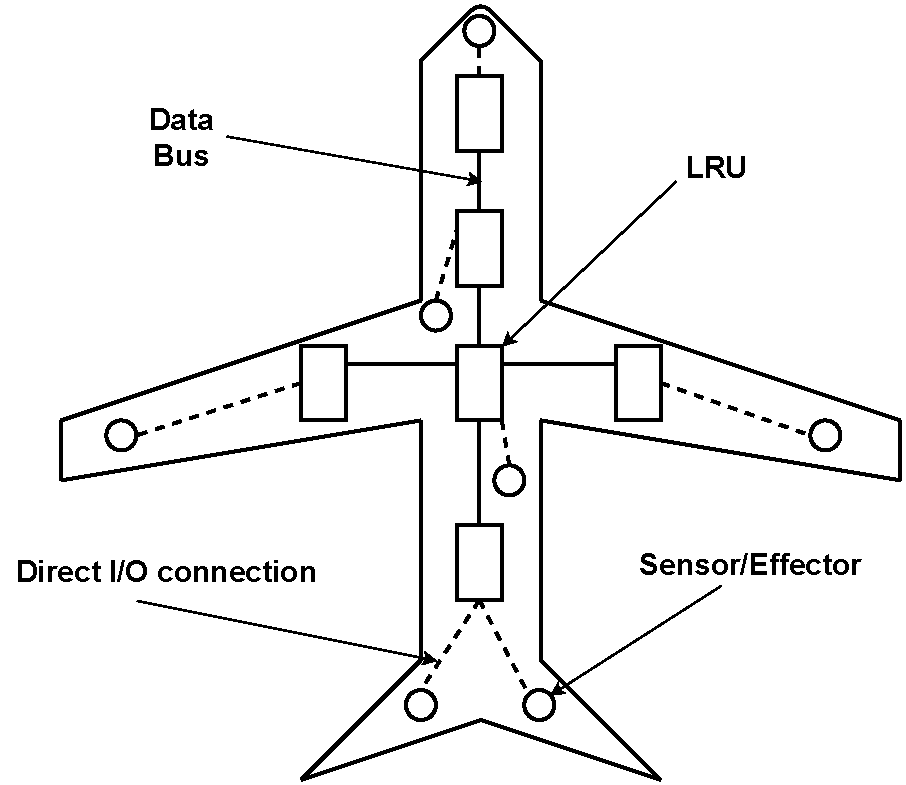
\includegraphics[width=1.0\textwidth]{figures/federated_architecture.pdf}
    \caption{Simplified visualization of the federated avionics architecture, showing \gls{lru}, sensors, effectors, and the global data bus}\label{fig:federated_architecture}
\end{figure}
\begin{figure}
    \centering
    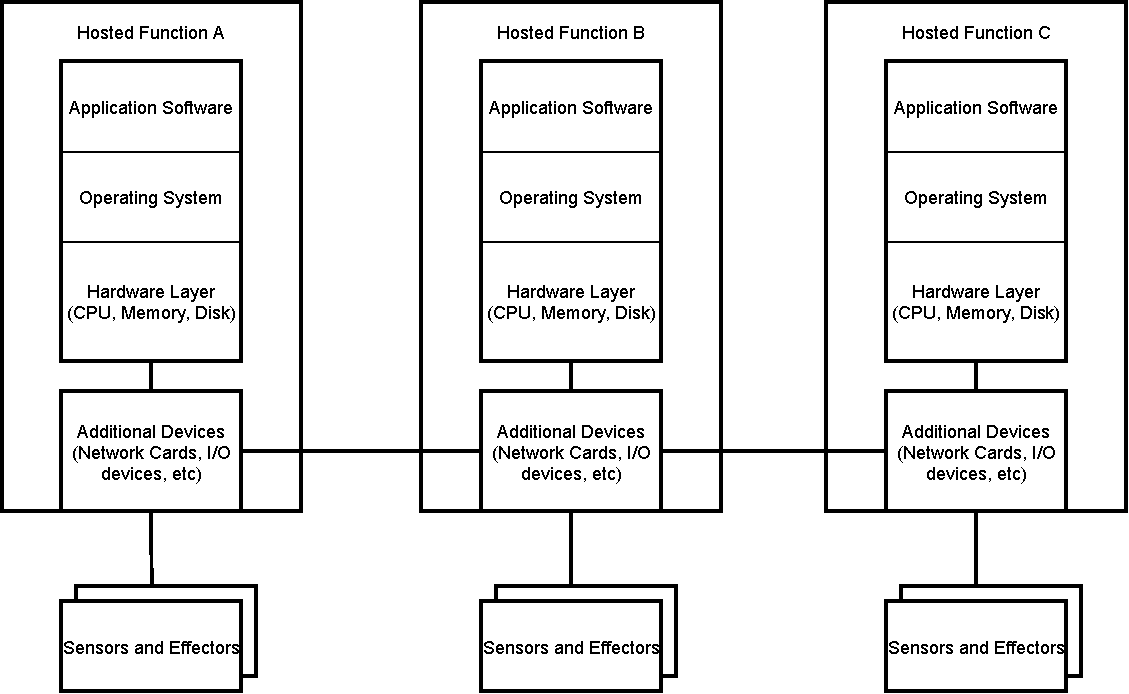
\includegraphics[width=1.0\textwidth]{figures/federated_architecture_components.pdf}
    \caption{Internal system architecture and interaction between \glspl{lru}}\label{fig:federated_architecture_components}
\end{figure}

\section{Integrated Modular Avionics}\label{section:integrated_modular_avionics}
\glsfirst{ima} is the direct successor of the federated avionics architecture. The idea behind \gls{ima}
is to consolidate the distributed hardware in one central flight cabinet. A Flight cabinet is very similar
to a rack in a datacenter. They can host multiple processing units, each comes with its own hardware stack
consisting of a \gls{cpu}, \gls{ram}, disk space and connectors for input and output\cite{prisaznuk1992integrated}. These servers are then plugged-in 
into the flight cabinet. Each server can host more than one avionic function and each function is allocated on partitions.
Partitions can be created on different ways and has been standardized in \gls{arinc653}\cite{vanderleest2010arinc}. The most common approach
is the use of a hypervisor (how this is implemented is being discussed in \autoref{section:workload_partitioning_strategies}). 
The flight cabinet provides power and required network connection to the plane's global data bus
as described in \gls{arinc629}\cite{isik2010arinc} or \gls{arinc429}\cite{fuchs2012evolution}. \gls{arinc629} is the successor of the data bus \gls{arinc429}.
Effectors and sensors communicate with the flight cabinet over \gls{arinc629}\cite{prisaznuk1992integrated}.
Sensors or effectors that are incompatible with \gls{arinc629} may communicate over remote data concentrators. Remote data concentrators are gathering data from sensors
or sending data to effectors over traditional \gls{io} connections. The gathered data or the received actions are communicated via \gls{arinc629} or \gls{arinc429}. Therefore,
remote data concentrators act as bridges between such devices and the data bus.
Using a central flight cabinet cannot replace all \glspl{lru} in the plane\cite{watkins2007transitioning}. These \glspl{lru} needs to be either integrated into the flight cabinet
or connected to the global data bus, for example via remote data concentrators. \autoref{fig:ima} depicts a simplified view on integrated modular avionics architecture in a plane.
The number of \glspl{lru} has been reduced and one central flight cabinet has been introduced. Remote data concentrators are working as bridges between sensors and effectors incompatible
with the data bus standard and the hosted functions in the flight cabinet. \autoref{fig:ima_components} shows the modules inside of such a flight cabinet. The flight cabinet
possesses multiple processing units. Each processing unit is comparable to a dedicated computer with its own hardware and operating system. These processing units
are being connected via a network layer and each processing unit hosts one or more hosted functions. Hosted functions are isolated from each other and have
a fixed predetermined set of resources and execution time.

\begin{figure}
    \centering
    \includegraphics[width=1.0\textwidth]{figures/ima.pdf}
    \caption{Simplified visualization of the integrated modular avionics architecture, showing sensors, effectors, cabinets and the data bus \glspl{lru}}\label{fig:ima}
\end{figure}

\begin{figure}
    \centering
    \includegraphics[width=1.0\textwidth]{figures/ima_components.pdf}
    \caption{View into a flight cabinet}\label{fig:ima_components}
\end{figure}

This system architecture has numerous advantages over the federated avionics architecture. Due to the more centralized approach \gls{ima}
is able to reduce weight via better cable management and less distributed processing units. Computing resources can be used more efficiently
via hosting multiple avionics functions on one processing unit. This leads to a higher system saturation. A positive side effect is less
energy consumption and a smaller ecological footprint. The reduced weight creates more space for cargo, fuel or passengers. 
Hardware consolidation leads to a consolidation of development efforts, which achieves cost and time savings\cite{watkins2007transitioning}.
The common processor allows the developer to focus on the hosted avionic function, enabling a better development experience and less error-prone
flight software. Separating software and hardware is a benefit during the certification process, because the certifying authority can certify
software and hardware separately. This has just another huge impact on cost and time savings. Additionally, upgrading the hosted function
becomes a lot easier, because of the hardware and software separation and less expensive hardware, due to standardized and more common
processing units. Another important benefit can be achieved via adopting the idea of open software and hardware. An open system architecture
with open standards can lead to a more competitive market due to industry-wide participation and exchangeability between hardware or
software applications. This way development and hardware costs can be reduced, because development cost gets distributed among all contributing
companies and mass production of standardized and open hardware shrinks marginal costs\cite{black2006open}. Moreover, the decoupling between hardware and software
can have a positive effect on new emerging companies, considering the lower costs\cite{watkins2007transitioning}. Software virtualization makes it easier to develop the
software, without buying expensive physical development kits. The software is being virtualized, tested and can be much later evaluated on real hardware, speeding up
the development process and time to market.

\section{Distributed Integrated Modular Avionics}\label{section:distributed_integrated_modular_avionics}
While \gls{ima} introduced a central architecture via consolidating computing resources into one central flight cabinet
\gls{dima} takes a different approach. \gls{ima} has shown that it is able to successfully reduce the number of components
in the plane with increasing number of hosted functions, because of its shared hosting infrastructure\cite{fuchsen2009preparing}.
Although this had positive effects on weight and cost management, there is room to improve in form of cable management.
Due to the centralized architecture it is necessary to connect every sensor and effector in the plane with the central flight cabinet
in the fuselage\cite{mccabe2009avionics}. This possible increase of cable length can be prevented via using ideas from the federated avionics and \gls{ima}.
\gls{dima} suggests a distribution of processing units, while taking into account the advantages of a central flight cabinet.
Instead of one central flight cabinet it is possible to redistribute the avionics functions over multiple flight cabinets distributed
in the plane's fuselage (see also \autoref{fig:dima}). This way it is possible to successfully exploit the advantages of the integrated architecture, while achieving
further improvements in the cable management\cite{li2012avionics}. Cable management is not the only possible adjustment for improvement.
The commercial cloud computing industry experienced a huge success over the last couple of years and these achievements can be used
for creating synergies between these two areas and applying cloud computing ideas in \gls{dima}. According to the \gls{nist} cloud computing is defined as:
\begin{displayquote}
\enquote{Cloud computing is a model for enabling ubiquitous, convenient, on-demand network access to a shared
pool of configurable computing resources (e.g., networks, servers, storage, applications, and services) that
can be rapidly provisioned and released with minimal management effort or service provider interaction.}\cite{mell2011sp}
\end{displayquote}
Although not all aspects of cloud computing are applicable on aviation, some of these aspects are.
One of these aspects is the separation into different service layers:
\begin{itemize}
    \item \gls{saas}
    \item \gls{paas}
    \item \gls{iaas}
\end{itemize}
\gls{saas} is handling all applications. \gls{paas} is responsible for the platform, where these applications
are running on (for example a hypervisor or services like webserver or databases). \gls{iaas} is the underlying
infrastructure (server, storages, networking). These three layers can be mirrored on the aviation world as follows:
\begin{itemize}
    \item \gls{saas}: Hosted functions
    \item \gls{paas}: The virtualized processing units or separation kernels
    \item \gls{iaas}: flight cabinets, remote data concentrators, the plane's data bus
\end{itemize}
Via separating each of these layers the aviation industry gains stronger standardization, more reliability and more effective
development workflows. Instead of selling one big monolithic system, separating makes it possible to develop products
for specific layers and interconnect them with the other layer via standards. These standards can be, as shown in \autoref{section:integrated_modular_avionics},
drivers for competition and exchangeability. Another aspect of cloud computing is the free and configurable allocation of applications\cite{li2012avionics}.
Dedicated storage, processor or sensor clusters would allow on-demand access from applications. Nevertheless it is a challenge to make this access reliable
and safe. Furthermore using standardized software may allow
interconnection between the plane and ground units (for example: real-time weather data transmitted from the ground to the plane).
This is partly comparable to the tactical data link of military units that get real-time radar data on their \gls{hsd}.

\begin{figure}
    \centering
    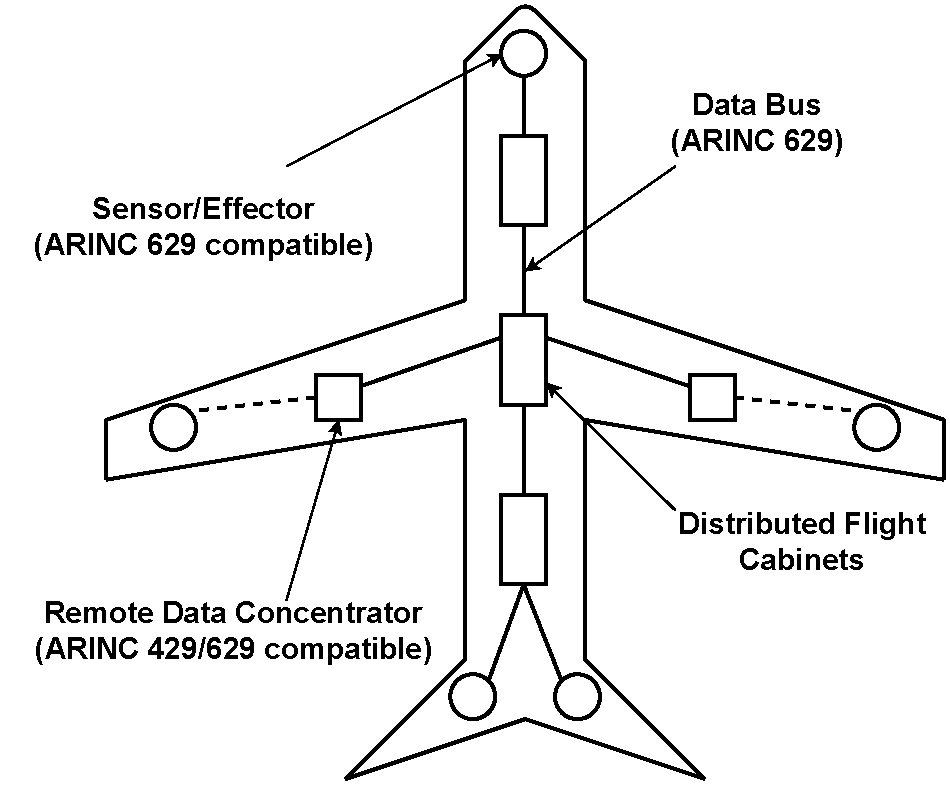
\includegraphics[width=1.0\textwidth]{figures/dima.pdf}
    \caption{Visualization of distributed flight cabinets}\label{fig:dima}
\end{figure}

\section{Workload Partitioning Strategies}\label{section:workload_partitioning_strategies}
Planes are composed of complex distributed systems with different tasks, requirements and environmental influences.
Every system has its own set of risks and possible impacts.
These different risks are known as \gls{dal} or \gls{idal} and have been defined
in the \gls{arp4754} as follows\cite{arp4754a2010guidelines}:
\begin{description}
    \item[A] Catastrophic system failures
    \item[B] Hazardous system failures
    \item[C] Major system failures
    \item[D] Minor system failures
    \item[E] No safety effect    
\end{description}

Due to these different risk levels it becomes important to isolate systems from each other. A system
with a low risk level should never have direct nor indirect impact on another system. In conclusion
the following measures are necessary to satisfy the safety and security requirements in planes:

\begin{itemize}
    \item Reserved \gls{cpu} time
    \item Reserved memory
    \item Reserved disk space
    \item \gls{qos}
    \item Network isolation
    \item Process isolation
    \item Privilege dropping
\end{itemize}

Reserved \gls{cpu} time means that every task has a strict time partition to work with.
Normally, cpu time is being shared on single processor systems. The operating systems simulates
parallelism via fast context switches. Multiple tasks are being executed consecutively switching
between them. This creates the impression that the system behaves parallel, but in reality it does not.
On multi processor systems real parallelism is possible. Reserved memory refers to a fixed memory
partition in the \gls{ram}. Reserved disk space refers to guaranteed space on a hard disk for storing
persistent data. Network isolation and Process isolatio ensures a noisefree and secure runtime environment.
Processes should not be disturbed by other processes either on process or network level. Furthermore,
each process has to drop privileges. Dropping privileges increases the safety and security of a service,
because it is less likely to interfere with other processes if the process has no privileges to do so.
\gls{qos} gives certain processes wit higher importance or risk level a higher priority. For example,
a system that controls the radar should have a higher priority than a system that just controls
the ambient lights in the passenger cabin.
Many of the above mentioned measures reveal other measures as direct dependencies. For example,
it is not possible to do proper \gls{qos} without an observable system that gets properly monitored.
Another example is the importance of security. On the first view security might be untangled of safety,
but in reality safety and security have a direct effect on each other. If the system is insecure it cannot
be safe and reliable, because every possible security incident could undermine all reliability promises.
The same applies to safety. An unsafe and unstable system cannot be considered secure, because these
weak points in the reliability might weaken the security. Just imagine a system that controls
permissions or security related functions. The system itself may be secure, but if it is unreliable 
it may has a direct effect on the security of other systems that depend on this particular system.
Additionally, planes have further constraints and requirements on software. One of these requirements
is a guarantee on response. Certain software systems in planes must respond before a given deadline.
This is called real-time communication. Real-time communication breaks down into the following types\cite{worn2006echtzeitsysteme}:

\begin{description}
    \item[Hard] The system has to satisfy all constraints. Responses are always on time. If a response would come too late it would inflict damage.
    \item[Firm] Executed tasks are worthless when their response does not satisfy the time constraint. No damage happens.
    \item[Soft] There are time constraints for requests and responses, but a tolerance exist. Delays are acceptable (as long as they fit in a specific time frame).
\end{description}

With all of these requirements it is obvious that there need to be technical implementations to satisfy all constraints.
The real-time constraints can be satisified via implementing real-time capabilities on operating system or kernel level.
Prominent examples are VxWorks' real-time operating system\cite{vxworks}, FreeRTOS\cite{freertos} or the real-time patches for the linux kernel\cite{realtimelinux}.
All other requirements are being solved either via virtualization or via containerization. There are two types of virtualization: Full virtualization and paravirtualization.
While full virtualization creates an almost full virtualized hardware including virtualized memory or \gls{io} devices, the paravirtualization does only virtualize
the software layer. The hardware stack will not be virtualized. Although this approach increases performance it is considered as less secure. With virtualization
it is possible to successfully isolate processes from each other and provide a dedicated workload partition for a specific software with its own \gls{ram} and \gls{cpu}.
The key element in this approach is the hypervisor. The hypervisor is the abstraction layer between the hardware, the software and their virtualized counterpart. 
Type 1 hypervisors run directly on the hardware, while type 2 hypervisors are running
on a dedicated host OS. Both hypervisors can usually virtualize a finite number of guests (finite, because the hardware resources are finite). Guests can be either applications or whole operating systems.
Many hardware provide direct support for virtualization, such as special instruction sets for \glspl{cpu}.
Containerization uses operating system or kernel level features to isolate processes or resources. In the Linux kernel this usually works via
making use of namespaces, kernel capabilities, control groups, union file systems and additional kernel features such like the \gls{ebpf}. Linux namespaces have been heavily influenced by namespaces in Plan 9 (an alternative
operating system by Bell Labs) and zones in Solaris. Contrary to traditional virtualization, namespaces do not need a hypervisor layer, instead the kernel offers
a single system call called \emph{setns()}\cite{mannamespaces}. The Linux namespace \gls{api} consists of six dedicated namespaces, each responsible for a different isolation environment\cite{namespacelist}:
\begin{description}
    \item[mnt] responsible for filesystem mount points
    \item[pid] responsible for processes
    \item[net] responsible for the network stack
    \item[ipc] responsible for \gls{ipc}
    \item[uts] responsible for \gls{uts}
    \item[user] responsible for \glspl{uid}
    \item[cgroup] responsible for \glspl{cgroup}
    \item[time] responsible for time  
\end{description}
The first namespace \emph{mnt} specifies the filesystem hierarchy for the isolated process or a group of processes. With this namespace it is possible
to mount only a specific directory structure into the isolated environment. This ensures that a process from environment \emph{A} cannot
access files on the host system or in another environment. The \emph{mnt} namespace has become especially useful in combination with union file systems.
Union file systems are layered filesystems and allow to mount multiple directory structures over each other. Docker uses this technology for combining
different layers to a full docker container image. The second namespace \emph{pid} gives the system the opportunity to run multiple processes 
with the same \glspl{pid} on the host system. Running multiple processes with the same \gls{pid} on one system fulfills different purposes.
On one hand this provides reliability across different hosts. Via this approach it is possible to run a process with the same \gls{pid} in different
environments on different physical hosts. On the other hand it provides isolation. The process can only see other processes contained in the same namespace\cite{lwnnamespace}.
The \emph{net} namespace is responsible for everything network related. It provides the isolated environment with \gls{ip} addresses, ports, routing tables
and virtual network devices. \emph{net} is mostly being used for isolating network connections from each other. For example a namespace \emph{A} could provide
its own ports and internal IP addresses, while a namespace \emph{B} could provide the same port. The ports can be forwarded to the host via port-forwarding.
The \emph{ipc} namespace handles everything \glsfirst{ipc} related (message queues, Linux signals like \emph{sigkill} for killing processes etc).
For dealing with different hostnames in different namespaces the \emph{uts} namespace is being used. The last three namespaces implemented by Linux
are the \emph{user}, \emph{cgroup} and \emph{time} namespaces. \emph{user} is responsible for \glsfirstplural{uid} and \glsfirstplural{gid}. With
the namespace \emph{user} it is possible to different users or groups with the same \glsplural{uid} or \glsplural{gid} in different environment.
For example, having the \emph{root} user (the administrator account on Linux systems) in different isolated environments. The user \emph{root}
is identified by the \gls{uid} 0 and the \gls{gid} 0. Different times in isolated environments are provided by the \emph{time} namespace.
The last namespace, the \emph{cgroup} namespace, is responsible for the \glsfirstplural{cgroup}. A \gls{cgroup} enables the system to limit
and monitor resources inside of a namespace via providing a pseudo-filesystem called cgroupfs\cite{mancgroups}. Each \gls{cgroup} consists
of one or more processes and each process is being modified by a subsystem (also known as resource controller). Subsystems work as modifiers
for these processes. Via these modifiers it is possible to set specific limits or monitor the processes. For example, limiting the available
\gls{cpu} time or memory for a process, increasing the priority for network traffic, limiting access to \gls{io} devices or
monitoring events created by a process\cite{mancgroups}. The last two missing building blocks for secure containers are kernel capabilities and the \glsfirst{ebpf}.
Kernel capabilities provide a more granular access to kernel features such like mounting or creating ports\cite{dockersecurity}.
Common kernel capabilities are \emph{CAP\_CHOWN} (changing the owner and group of a file), \emph{CAP\_NET\_BIND\_SERVICE} (allow the binding of ports under 1024), 
\emph{CAP\_SYS\_ADMIN} (allow system administrator access), \emph{CAP\_NET\_ADMIN} (allow network administrator access, a complete list can be found
in the corresponding man page for kernel capabilities\cite{mancapabilities}). The \glsfirst{ebpf} is the successor of the \glsfirst{bpf}. The \gls{bpf} is 
well known for its human readable filtering language that allows filtering, monitoring and analyzing packets in computer networks. Core of the \gls{bpf}
is a \gls{jit} compiler that translates the human readable \gls{bpf} language into machine readable byte code. Contrary to its predecessor, \gls{ebpf} is not limited
to network packets. With Linux version 3.18, \gls{ebpf} has been embedded into the Linux kernel as virtual machine and allows filtering for any sort of \glsfirst{ipc},
such like socket connections, system calls (syscalls) or kernel permission delegations. \autoref{fig:workloads} gives an overview over different workload partitioning and
deployment techniques. On the far left is the traditional setup with the hardware, an operating system running on the hardware, the applications and their shared libraries.
The second pillar shows a type 2 hypervisor with a hardware, an operating system, shared libraries on the operating system, a hypervisor and virtual machines. Each virtual machine
comes with their own operating system, shared libraries and the actual payload (the application with the workload). The type 1 hypervisor simplifies this setup with running
a hypervisor directly on the hardware. In this case, the hyperviso is hypervisor and operating system at once. The container deployment comes with the hardware, an operating system 
and its shared libraries, a container runtime for running containers and containers running
in this container runtime. Each container can consist of different parts. A container can consist of only one static built executable or an application and shared libraries.
Shared libraries minimize the size of software via sharing common methods, for instance a library for \glsfirst{rpc} or \gls{dns} lookups. When the executable has been linked dynamically,
the executable can dynamically look up these common methods.
Contrary to dynamic linking is static linking, where a software is being compiled with all its dependencies into one executable. Although all deployment techniques may look similar at a first glimpse,
they are indeed completely different. A virtual machine allows stricter isolation compared to running all applications without virtualization and a container can consist of a single binary.
\begin{figure}
    \centering
    \includegraphics[width=1.0\textwidth]{figures/workloads.pdf}
    \caption{Overview over different workload partitioning and deployment techniques}\label{fig:workloads}
\end{figure}

\section{Challenges and Opportunities}\label{section:Challenges_And_Opportunities}
Prior, this thesis has explored past, present and future avionic system architectures. On the next pages it is going to examine
challenges in these avionic system architecture designs and possible enhancements in the avionic domain in general. This document is explicitly ignoring the certification
process of software. It is known that a certification process in the avionic domain can be slowly and very costly, due to its
high risk to passengers, flight personnel and civilians on the ground. Enhancing this certification process via altering the certification itself, while matching the right balance between safety
and development speed or costs, is explicitly not topic of this research. Instead, this document tries to focus on few main questions.
The first identified challenge is the increase of development speed in the avionic domain. Pushing innovations and new technologies fast are a major
success factor. Maintaining a hardware and software stack for a traditional avionic system architecture, like the federated architecture, is a
huge cost and time disadvantage. The developer cannot use the standard development tools and needs to adapt to the new environment. Moreover,
buying the necessary equipment and constantly adjusting the software to this equipment are toilsome and complicated. Every hour of additional
work is a cost factor that leads to higher unit prices, smaller profit margins and less time for more features. Costs directly lead to the next
challenge: Decreasing development costs and increasing feature output. Considering the tight entanglement of soft- and hardware in federated systems
these stacks become very cost intensive. Also, the feature output is limited to the required hard- and software,
hence limiting possible performance or functionality gains. Performance is another challenge. As a result of heavy use of virtual machines the performance
gains are not as high as they could be. The hard- and software limitations make the system less extensible and less adjustable. Another challenge is the
proprietary avionic system development environment. Proprietary standards, hardware- and software have devastating effects on innovation, safety, security,
costs and technological development. Innovation is affected negatively, because of less communication between companies. Open architectures, software or hardware
increase communication and share knowledge between all development entities. These shared knowledge and improved communication is known for increasing
security of software\cite{hoepman2007increased}. Restricting access to the source code may help restricting the attacker's knowledge for executing attacks, but it is shown that
``keeping the source code closed appears to be difficult''\cite{mercuri2003security}. Furthermore, patches for open source software are released twice as fast
as for closed source software\cite{witten2001does}. The increased pace of patching the software underlines the increased development speed and its connected
benefits. Many of the highlighted challenges are not new for the tech industry. The cloud industry has solved several of these challenges successfully.

\chapter{Cloud-Native}
\section{Introduction}
Containers are not a new concept. The idea behind them goes back to systems like Solaris, FreeBSD or Linux. FreeBSD has released their first container-alike
isolation environment, called \emph{jails}, in 2000\cite{FreeBSD4Announcement}. Jails is heavily being influenced by the chroot system call on Unix systems.
The chroot system call has been introduced with Version 7 Unix in 1979\cite{BYTE}. The concept has been there all the time so what was missing?
Although containers were in use by system administrators the workflow was not developer friendly enough. Big companies like Google
realized the potential of containers early and started to heavily use them in their own infrastructure, but the overall success
came with open source technologies like Docker or Kubernetes. It turned out that opening up the development process of these technologies
has been the perfect foundation for creating a community that spans over several companies and industry branches. This community is under
supervision of the Linux Foundation and is called \glsfirst{cncf}\cite{CNCFFounding}. The \gls{cncf} built an enormous ecosystem for
running and orchestrating containers. \autoref{fig:landscape} visualizes the scale of the \gls{cncf} related projects\cite{CNCFLandscape}. Considering that
that the \gls{cncf} was founded in 2015 this is clearly a huge success for the containerization of applications in different industry branches, especially
for the cloud computing industry. Looking at the landscape it can be seen that the \gls{cncf} covers different areas and expands wide beyond containerization.
Just to name a few different areas and their sub areas on the landscape:

\begin{description}
    \item[App Definition and Development] databases, streaming and messaging, application definition and image build, continuous integration and delivery
    \item[Orchestration and Management] scheduling and orchestration, coordination and service discovery, remote procedure call, service proxy, api gateway, service mesh
    \item[Runtime] cloud native storage, container runtime, cloud native network
    \item[Provisioning] automation and configuration, container registry, security and compliance, key management
    \item[Observability] monitoring, logging tracing, chaos engineering
\end{description}

While some of the above areas play only a minor role in the aviation industry some areas are usable or will play a bigger role in the future.
Especially, areas like scheduling and orchestration or container runtime are from interest for the aviation industry, because
these areas provide related functionality compared to current solutions in actual use within the aviation industry.

\begin{figure}[H]
    \centering
    \includegraphics[width=1.0\textwidth]{figures/landscape.png}
    \caption{Cloud Native Computing Foundation Landscape}\label{fig:landscape}
\end{figure}
 
\section{Docker}
Docker (released in 2013\cite{DockerRelease}) has revolutionized the way containers are being used.
Before Docker, the primary users of containers have been sysadmins, who used containerization to isolate environments from each other. With Docker
this workflow has changed. Docker has introduced a unique file format, called Dockerfile, for describing a container consisting of different layers. These layers
are stacked on each other, with the help of union file systems, for a final Docker image. This process has a few advantages. Each layer can be cached separately, leading
to less disk usage and faster container build times. Layers do not need to be from the same author. In Docker it is very common to re-use common Docker images
as a base layer and add additional payload to them via adding layers on top of the base layer. The base layer is often called the base image and the most popular
base image is the \emph{scratch} image. \emph{Scratch} is just an empty Docker layer. All other base images use the \emph{scratch} image as start point for the build process.
Base images can be whole Linux distributions like Debian, proprietary operating systems from the industry or just a directory structure. For example, Google provides
a \emph{distroless} Docker image that just contains time zone data and the global certificate chain\cite{Distroless}. The \emph{distroless} image is mainly in use for shipping
static binaries inside of Docker. This is common practice for languages like Rust or Go. Shipping just the binary leads to a much smaller attack surface. Having no shell inside
of the image makes it impossible for an attacker to gain shell access to such a container and missing additional executables make it difficult to
exploit additional executables for building an attack chain (for example via using network utilities for opening a reverse shell into the container).
\autoref{lst:dockerfile} shows an example multi-stage Dockerfile with different layers. Each line in the file is a separate layer in the final image
and each \emph{FROM} statement defines a different stage in the docker image build process. In the first stage of the Dockerfile
a small hello world program will be written in the programming language Go (often referred to as Golang) and compiled. In the second stage,
the executable from the first stage will be copied to the new second stage, placing it into a \emph{distroless} image for reducing the possible
attack surface and making the executable available for further distribution as docker image. The first stage starts with the statement
\emph{FROM docker.io/golang:1.17 AS GO\_BUILD}, setting the base image to \emph{golang} with version 1.17 from the docker registry \emph{docker.io}
and naming this stage \emph{GO\_BUILD}. A docker registry is a public or private repository for docker images. 
The second statement \emph{WORKDIR /go/src/app} sets the working directory for the build process. It is comparable to moving to a folder
in a Windows system or changing the directory in a Linux system via the command line command \emph{cd}. The next three statements starting
with \emph{ENV} are setting environment variables. Environment variables are an operating system feature for setting variables outside
of programs for configuration purposes. \emph{GOOS} sets the target operating system to Linux, \emph{GOARCH} sets the architecture to amd64
and \emph{CGO\_ENABLED} disables the libc support for the Go build process. Disabling the libc support is equal to disabling linking
to shared libraries, resulting to a static compiled binary that can be moved on different systems as long as the target operating system
and architecture stays the same. With the next three \emph{RUN} statement it is possible to execute commands in the base image
\emph{docker.io/golang:1.17} (this also means that our base image is actually based on Linux). The \emph{echo} command
prints our Go hello world code and pipes it into a file called \emph{main.go}. Using \emph{go mod init app} initializes
the Go build and dependency system with a name for the app. Running \emph{go build -o /out/app .} will build the \emph{main.go}
file in the current directory and move the created executable \emph{app} to the directory \emph{/out/}. Using the next
\emph{FROM gcr.io/distroless/base} statement a new stage will be build with a new base image for the final image holding the executable
and reducing possible attack surface by utilizing Google's \emph{distroless} images. The \emph{COPY} statement will
copy the built executable from the first stage into the new second stage and the \emph{ENTRYPOINT} statement will set
the path of the application as entrypoint for the container startup. It is important to differ between images and containers.
Containers are running instances of images. The entrypoint is the start point from each container and be compared to the main function
of most C-alike programming languages or the init system of a modern operating system. \autoref{lst:dockerbuild} shows
the output of building the docker image. Each step is equal to one layer of the final image and each layer has a unique
\gls{sha256} checksum over the binary content of the layer for ensuring integrity and reproducibility. This minor information
has a unique impact on supply chain security, developer experience and costs, because with each layer cryptographically
identified it is much more difficult to tamper with the build process, allowing secure access to cached layers
and leading to faster development speed and lower costs. The final image can be run as container via executing
\emph{docker run} leading to the promised \emph{Hello World!} line. 
\begin{minipage}{\linewidth}
\begin{lstlisting}[caption={A multi stage Dockerfile with different layers},label={lst:dockerfile}]
FROM docker.io/golang:1.17 AS GO_BUILD
WORKDIR /go/src/app
ENV GOOS=linux
ENV GOARCH=amd64
ENV CGO_ENABLED=0
RUN echo "package main\nimport \"fmt\"\nfunc main() { fmt.Println(\"Hello world!\") }" > main.go
RUN go mod init app
RUN go build -o /out/app .

FROM gcr.io/distroless/base
COPY --from=GO_BUILD /out/app .
ENTRYPOINT ["./app"]
\end{lstlisting}
\end{minipage}
\begin{minipage}{\linewidth}
\begin{lstlisting}[caption={Output of a docker build run with shortened SHA256 checksums},label={lst:dockerbuild}]
STEP 1: FROM docker.io/golang:1.17 AS GO_BUILD
STEP 2: WORKDIR /go/src/app
--> Using cache baa3b5061ca
--> baa3b5061ca
STEP 3: ENV GOOS=linux
--> Using cache fe142d360ee
--> fe142d360ee
STEP 4: ENV GOARCH=amd64
--> Using cache 49771a6a4a6
--> 49771a6a4a6
STEP 5: ENV CGO_ENABLED=0
--> Using cache edf307d8374
--> edf307d8374
STEP 6: RUN echo "package main\nimport \"fmt\"\nfunc main() { fmt.Println(\"Hello world!\") }" > main.go
--> Using cache ca435b8adf9
--> ca435b8adf9
STEP 7: RUN go mod init app
--> Using cache 19b7a23f24d
--> 19b7a23f24d
STEP 8: RUN go build -o /out/app .
--> Using cache baeee09e19f
--> baeee09e19f
STEP 9: FROM gcr.io/distroless/base
STEP 10: COPY --from=GO_BUILD /out/app .
--> Using cache 5ab01f9acf7
--> 5ab01f9acf7
STEP 11: ENTRYPOINT ["./app"]
--> Using cache 288ac81c34b
--> 288ac81c34b
\end{lstlisting}
\end{minipage}
\section{Open Container Initiative}
In June 2015 leading container projects, such like Docker and CoreOS (a minimal Linux distribution for running containers), launched the \gls{oci}
under auspices of the Linux Foundation\cite{OCIabout}. The \gls{oci}'s purpose is the standardization of Docker's container image specification (image-spec\cite{ImageSpec}), container runtime (runtime-spec\cite{RuntimeSpec})
and content distribution (distribution-spec\cite{DistributionSpec}). These three specifications address everything from building a container image, distributing the image
over a container registry, and running the container. Standardization enables interchangeability of all three implementations and increases possibilities for their production usage.
In the following, this thesis will have a short glimpse on each of the specifications. A full writeup would break the constraints of this thesis. It is recommended to read
the original specification, if more information is needed. The image specification has five essential components:

\begin{description}
    \item[manifest] provides a set of layers and a configuration for a specific image runnable on a specific architecture and operating system
    \item[image index] provides a set of manifests with different architectures and operating systems
    \item[image layout] provides a file system layout (the contents of the image) 
    \item[filesystem layers] provides information about merging different layers to one image
    \item[configuration] provides the configuration of the image, provided by the Dockerfile (environment variables, entrypoints, etc)
\end{description}

\autoref{lst:imageManifest} depicts a very simplified example image manifest. The \gls{sha256} checksums have been shortened for saving space in this document.
The manifest shows the schema version, a configuration, multiple layers and annotations. The configurations and layers have media types, a field for the
size and a digest (a checksum) of the addressable content. Annotations provide further information for the image. The \gls{oci} manifest specification
defines a few predefined annotations, but at last these are just customizable strings. Annotations allow additional metadata for images, thus
providing information for various other use cases, like easier search in an \gls{oci} compatible registry or information about its maintainers.
With the manifest it is possible to address the content via its offset and to provide integrity via digests \cite{ImageManifestSpec}. One or more image manifests can form
an image index. An image index is a set of different image manifests for different operating systems and architectures \cite{ImageIndexSpec}. \autoref{lst:imageIndex} illustrates
such an image index with support for two platforms. The first addressed manifest links to a manifest for MacOS with M1 chipset. The second addressed manifest
refers to a manifest for Linux with amd64 chipset. Furthermore, it is possible to add additional annotations to the image index definition. As mentioned earlier,
an \gls{oci} image consists of different layers. These layers are defined in the image layout and the filesystem layers specifications. One or more compressed layers are applied
on top of each other to create the entire root filesystem of the image\cite{ImageFSSpec}. The filesystem layers specification can handle 
additions, modifications and removals of various file types, such like directories, sockets, symbolic links, block devices, or regular files\cite{ImageFSSpec}.
All of these layers are described as an image layout. Each layer is stored in the image layout as \gls{blob} and addressable via its \gls{sha256} digest. An \gls{oci} image layout
is comparable to a directory in a filesystem. A \gls{blob} directory stores all layers, an index.json file provides platform interoperability via establishing the relationship
between each layer and their target platform \cite{ImageLayoutSpec}. \gls{oci} layout files work as marker and version identifier of the \gls{oci} layout. While the prior mentioned specifications
define the structure of the \gls{oci} image, the configuration specifies the environments, entrypoints, volumes, working directory, commands that should be executed and other configuration parameters.
The \emph{docker image inspect <docker image>} command prints a full OCI image configuration for a given image. \autoref{lst:imageConfiguration} shows the output of this command
for the prior mentioned OCI image, built from \autoref{lst:dockerfile}. The output has been cut down to the most important parts. Clearly visible are the environment in form of environment
variables, the command, the working directory, an entrypoint, the docker version, a build date and the root file system layers. If compared with \autoref{lst:dockerfile} the similarities are obvious. 
This image configuration works as interface for the runtime specification. The \gls{cri} provides an interface for running \gls{oci} compatible images. Common implementations of the \gls{cri} are
docker, containerd\cite{Containerd} or cri-o\cite{CRIO}. Containers are encoded as filesystem bundles. A filesystem bundle consists of the container configuration as specified in the \gls{oci} image specification
and the container's root filesystem (referenced in the image configuration)\cite{FilesystemBundle}. These filesystem bundles are executed by the container runtime. The container runtime manages the state and the lifecycle
of the container. Every container runtime implementation must fulfil the \gls{cri} specification's lifecycle operations and commands for basic runtime interaction (create, start, stop, kill, etc).
Distributing a container image is described by the \gls{oci} distribution specification. The distribution specification defines all necessary components of an \gls{oci} image compatible registry
and its basic operations. Described are the pull of an image (the act of downloading \glspl{blob} and manifests from the registry), the push of an image (the act of uploading \glspl{blob} and manifests to the registry),
and the registry itself. 

\begin{minipage}{\linewidth}
\begin{lstlisting}[caption={An OCI image manifest with two layers, shortened sha256 checksums and two annotations},label={lst:imageManifest}]
{
    "schemaVersion": 2,
    "config": {
        "mediaType": "application/vnd.oci.image.config.v1+json",
        "size": 8652,
        "digest": "sha256:b5bb9d8014a0f..."
    },
    "layers": [
        {
            "mediaType": "application/vnd.oci.image.layer.v1.tar+gzip",
            "size": 40270,
            "digest": "sha256:c739918a22764..."
        },
        {
            "mediaType": "application/vnd.oci.image.layer.v1.tar+gzip",
            "size": 14743,
            "digest": "sha256:9f767b0b078d2..."
        }
    ],
    "annotations": {
        "org.opencontainers.image.authors": "Christian Rebischke",
        "org.opencontainers.image.title": "A very easy manifest example"
    }
}
\end{lstlisting}
\end{minipage}
\begin{minipage}{\linewidth}
\begin{lstlisting}[caption={An OCI image index with multiple manifests, shortened sha256 checksums and platform specifications},label={lst:imageIndex}]
{
    "schemaVersion": 2,
    "manifests": [
        {
            "mediaType": "application/vnd.oci.image.manifest.v1+json",
            "size": 9783,
            "digest": "sha256:6650b51fab815ad7fc331f...",
            "platform": {
                "architecture": "arm64",
                "os": "darwin"
            }
        },
        {
            "mediaType": "application/vnd.oci.image.manifest.v1+json",
            "size": 9543,
            "digest": "sha256:ed22e9fb1310cf6c2decab...",
            "platform": {
                "architecture": "amd64",
                "os": "linux"
            }
        }
    ],
    "annotations": {
        "org.opencontainers.image.created": "2021-12-19T16:39:57-08:00",
    }
}
\end{lstlisting}
\end{minipage}
\begin{minipage}{\linewidth}
\begin{lstlisting}[caption={An OCI image configuration created via docker image inspect (shortened)},label={lst:imageConfiguration}]
{
    "RepoTags": [
    "hello-world:latest"
    ],
    "Created": "2021-12-19T07:47:29.318765235Z",
    "ContainerConfig": {
    "Hostname": "motoko.shibumi.dev",
    "User": "0",
    "AttachStdin": false,
    "AttachStdout": false,
    "AttachStderr": false,
    "Tty": false,
    "Env": [
        "PATH=/usr/local/sbin:/usr/local/bin:/usr/sbin:/usr/bin:/sbin:/bin",
        "SSL_CERT_FILE=/etc/ssl/certs/ca-certificates.crt"
    ],
    "Cmd": [
        "/bin/sh",
        "-c",
        "#(nop) ",
        "ENTRYPOINT [\"./app\"]"
    ],
    "Image": "sha256:bc721b69a6af4bb...",
    "WorkingDir": "/",
    "Entrypoint": [
        "./app"
    ],
    "DockerVersion": "20.10.12",
    "Architecture": "amd64",
    "Os": "linux",
    "Size": 22013044,
    "VirtualSize": 22013044,
    "RootFS": {
    "Type": "layers",
    "Layers": [
        "sha256:c0d270ab7e0db0...",
        "sha256:e3d24823466584...",
        "sha256:589f2bccf144b2..."
    ]
    },
}
\end{lstlisting}
\end{minipage}


\section{Container Interfaces}
With the rise of the \glsfirst{oci}, more and more container management systems and orchestration services have been developed.
While the implementations of the \glsfirst{cri} provides basic runtime functionality for executing containers, it became clear that
an interface for running containers is not enough. The usecases for containers became more complex and orchestration services became
distributed over large network topologies. This distribution lead to the necessity of standardized networking and storage interfaces.
These interfaces are called \glsfirst{cni} and \glsfirst{csi}. This section summarizes both interfaces and gives a good introduction.
However, this section is not meant as complete guide for implementing these interfaces. \glspl{csi} provide an interface for new storage providers.
A storage provider is the vendor of the plugin implementation\cite{CSISpec}. Storage providers can be providers for local or remote storage.
Every local storage differs and there are different ways on a system to provide storage for an application. Local Storage can be offered
via device mappers, the \gls{lvm}, raw block devices, volume groups or many other operating system and hardware dependent systems. Remote
storage equally complicated with additional network capabilities and protocols, such like \gls{nfs} or ceph (the distributed, fault-tolerant storage platform).
Each of these storage providers have a different \gls{api} and different ways to read and write data on them.
Container orchestrators implement the \gls{csi}. Communication between the \gls{csi} plugin and the container orchestrator happens over \gls{rpc}. The most common \gls{rpc} protocol
in the cloud-native environment is \gls{grpc}. \gls{grpc} (invented in 2016 by Google) has the huge advantage that it is language independent, supports a very
simple service definition via Protocol Buffers and bi-directional streaming with several security features like authentication\cite{GRPCConcepts}.
Protocol Buffers is an \gls{idl}. \glspl{idl} offer a, for the developer, convenient way to describe an \gls{rpc} interface in a language independent and
human-readable way. \gls{grpc} and Protocol Buffers are the tools of choice for the \gls{csi}. The \gls{csi} presents basic functionality for 
dynamic provisioning of volumes (on-demand provisioning), attaching or detaching volumes, mounting or unmounting volumes from an orchestration node, creating or deleting snapshots
or provisioning new volumes\cite{CSISpec}. Snapshots are one-time states of a volume with data, they are not equal to backups. Snapshots allow the storage provider
to go back in time and restore data for a given time frame. For this operation the storage provider requires necessary metadata and a running service. This is what
distances them from a backup. A backup offers a reliable way to restore a full dataset in case of a disaster (for instance a hardware outage). A snapshot does not
offer this reliability and may fail if the underlying system is damaged. Usually, a storage provider implements an \glsfirst{api} that is \gls{csi} compatible
or a third-party implements a service that interprets the \glspl{api} of the storage provider plugin and translates it, to be \gls{csi} compliant. When container orchestrators
like Docker became distributed over multiple nodes the network became more relevant. The \glsfirst{cni} specification addresses this problem and proposes a standard interface
for enhanced network capabilities for future container runtime and container orchestration solutions. Equally to the \gls{csi} specification, the \gls{cni} specification is language agnostic,
but the reference implementation is written in Go\cite{CNISpec}. As of writing this thesis, there are already over 20 \gls{cni} compatible plugins from various cloud providers, hardware vendors
or third-parties. These plugin differ significantly, because they address different use cases, problems or network environments. The \gls{cni} specification abstracts these differences and provides
a common interface for all of them. \gls{cni} plugins are not bound to one specific layer of the \gls{osi}. For instance, the \gls{cni} plugin \emph{flannel} focuses on \gls{osi} layer 3 only, hence providing
every container with its own unique routable \gls{ip} address via spanning an IPv4 network over all container orchestration nodes in a cluster (a cluster is a group of multiple orchestration nodes, responsible
for running containers or managing the cluster)\cite{Flannel}. Other \gls{cni} plugins such like \emph{cilium} or \emph{calico} offer support for more \gls{osi} layers and more features, such like
traffic encryption, traffic monitoring, network policies or more graduated network and routing capabilities.

\section{Kubernetes}
\subsection{Introduction and History}
Although Docker has been released in 2013, Google has been using Containers for a much longer period of time. According to Google engineers, they are managing Linux containers at scale since
at least 2006\cite{burns2016borg}. This long history of Linux container management lead to several internal container orchestration platforms within Google, such like Borg\cite{verma2015large}, Omega\cite{schwarzkopf2013omega} or Kubernetes\cite{kubernetesWebsite}.
While Borg and Omega are internal projects and therefore proprietary, Kubernetes is open source and freely available on GitHub\cite{KubernetesGithub}. Since the Kubernetes release in 2014\cite{KubernetesFirstRelease}, Kubernetes has started a chain reaction
in the industry. More and more projects have been founded around Kubernetes as distributed container orchestrator. The \glsfirst{cncf} landscape lists a plethora of different projects and project domains around Kubernetes, such like continuous integration and continuous delivery frameworks,
service proxies, service meshes, Kubernetes compatible container runtimes, \glsfirst{cni} or \glsfirst{csi} plugins or security addons for Kubernetes. This extensibility is one of Kubernetes' many success drivers. Kubernetes offers everything necessary for running
\gls{oci} compatible containers distributed on one or more Linux hosts, called nodes. These \gls{oci} compatible containers do not even need to be containers in the traditional sense. It is possible, with a little bit of effort and the KubeVirt project\cite{KubeVirt},
to run small virtual machines with Kubernetes. Such virtualized containers are called microVMs. However, on default Kubernetes focuses on running containers as abstracted by namespaces, cgroups and other Linux kernel features. Kubernetes does this
slightly differently to other container orchestrators. The smallest manageable unit in the Kubernetes world is being called a \emph{pod}. A pod consists of one or more containers and possesses a few additional properties to enhance container management and orchestration.
These differences will be explained in more detail in the following sections.

\subsection{Architecture}
\begin{figure}[H]
    \centering
    \includegraphics[width=0.8\textwidth]{figures/kubernetes.pdf}
    \caption{Overview over a Kubernetes cluster with three control nodes and three worker nodes}\label{fig:kubernetes}
\end{figure}
In this section, this thesis explores the architecture of Kubernetes. \autoref{fig:kubernetes} depicts a Kubernetes cluster with three control nodes and three worker nodes. Many control nodes form a control plane.
Control nodes are responsible for managing the cluster, while worker nodes are carrying the actual application payload. In case of an airplane the worker nodes could, for example, carry applications for controlling
the cabin temperature, lights or the entertainment system. Each node is connected to each other via a reliable and highly available network plane (symbolized by a switch in the middle). All nodes consist of a
an operating system (Linux) and a container runtime. The operating system is very often a highly specialized Linux distribution, for instance Flatcar Linux\cite{FlatcarLinux} or Fedora's CoreOS\cite{FedoraCoreOS}.
Specialized Linux distributions have the huge advantage of being very minimal, high secure and require low maintenancy. They accomplish this via only shipping the Linux kernel, an init and service daemon like systemd\cite{systemd}
and a very small read-only base system. System upgrades are conducted through ostree image updates. The ostree is the operating system tree containing the base system. Contrary to other traditional Linux distributions like Debian,
these specialized Linux container operating systems do not update software independently. Instead, the system upgrade is conducted via upgrading the whole base system at once. This procedure allows a very high testability, reliability
and a lower maintenance compared to traditional Linux distributions. On top of the operating system is the container runtime, popular container runtimes are containerd\cite{Containerd} or cri-o\cite{CRIO}. Docker was another famous
container runtime for Kubernetes clusters, but it got recently deprecated in favor of containerd\cite{KubernetesDockerNews}. Everything above container runtime level depends on the role of the node. Additional components of a control
node are an etcd\cite{etcd} instance, a kube-controller, a kube-scheduler and a kubeAPI instance. Etcd, is a highly available, reliable and distributed key-value store. Kubernetes uses etcd as its database for storing its actual 
and desired state. Every change on the Kubernetes cluster will be stored in the etcd cluster running distributed on all control nodes. Concensus is achieved via Raft, an advanced concensus algorithm proposed
by the Stanford University\cite{ongaro2013search}\cite{ongaro2014search}. Raft, that stands for replicant and fault-tolerant, implements consistency and partition tolerance as defined by Eric Brewer's CAP-theorem\cite{brewer2017spanner}.
Eric Brewer's CAP theorem states that a distributed system can only implement two of three properties of the CAP theorem. These three properties are consistency, availability and partition tolerance. Consistency is when each node
has the newest data, availability is when all read and write requests are always successful and partition tolerance means that the distributed continues to operate even when not all nodes are available\cite{bijlsma2020distributed}.
Raft guarantees consistency and partition tolerance, but it cannot guarantee availability due to unknown factors like network outages.  Instead of using time, Raft uses election terms and roles for each node. Everytime an election is held,
Raft will increment the term counter. On initialization all nodes have the role \emph{follower} and the term counter on each node is zero. The first election term begins with one follower nominating itself as \emph{candidate} and
advertising this nomination to all other nodes. The other nodes will react with an acknowledgement and the candidate node will be promoted to a \emph{leader}. The leader node sends heartbeats to every other node in the cluster.
When a cluster node receives such a heartbeat the node's timeout will be reset. As long as the leader stays healthy nothing happens and the cluster works as usual. As soon as the leader dies the other nodes will stop
receiving heartbeats. The missing heartbeart will lead to a timeout expiration. When this happens the expired node will increment the election term counter and nominate itself for a new leader and the process starts from new.
This process ensures the partition tolerance as defined by Eric Brewer's CAP theorem. Data can be added to the key-value store only through the leader node and all followers will forward write requests to the leader node. 
The message is considered committed as soon as the majority of nodes acknowledged the write operation. Read operations can be done on every node. This is equal to Eric Brewer's consistency property of the CAP theorem.

\subsection{Application Programming Interface (API)}
\subsection{KubeEdge}
\subsection{Impact on Reliability and Security}
\section{Secure Software Supply Chains}
\chapter{Cloud Native and Aviation}
\chapter{A first prototype}
\chapter{Conclusion}

\nocite{*}
\printbibliography{}
\lstlistoflistings{}
\listoftables{}
\listoffigures
\glsaddallunused
\printglossary{}
\end{document}
